
\section{IoT \& Big Data Platform}

Challenges of WAZIUP will be tackled using an open IoT-big data platform with affordable sensors connected through an IoT-Cloud open platform.
This platform will also make use of mobile phones and real-time processing to empower users and deliver the needed services.
The project will not develop any new IoT/Big Data software platform, but, rather exploit the existing solutions and adapt them for the purpose. Hereafter a compact list of core technical functionalities encompassed by the platform:

\begin{itemize}
   \item \emph{Cloud-based real-time data collection combined with analytics and automation software:} thus, the platform will offer cost-effective solutions for aggregating different machines and sensor types to engender efficiency, smart automation and optimization in the rural context.
   \item \emph{Intelligent analytics of sensor and device data:} studied in order to optimize for performance of the rural workplace, detect potential outages, and finally reduce overall maintenance costs.
   \item \emph{Integration to 3rd parties' platform:} enables customers' benefit of scaling fast and easy.
   \item \emph{PaaS (Platform-as-a-Service) provider:} WAZIUP will provide to business clientele with independently maintained platform upon which their web application, services and mobile applications can be built.
\end{itemize}

\subsection{Platform overview}


\begin{figure}[h!]
\centering
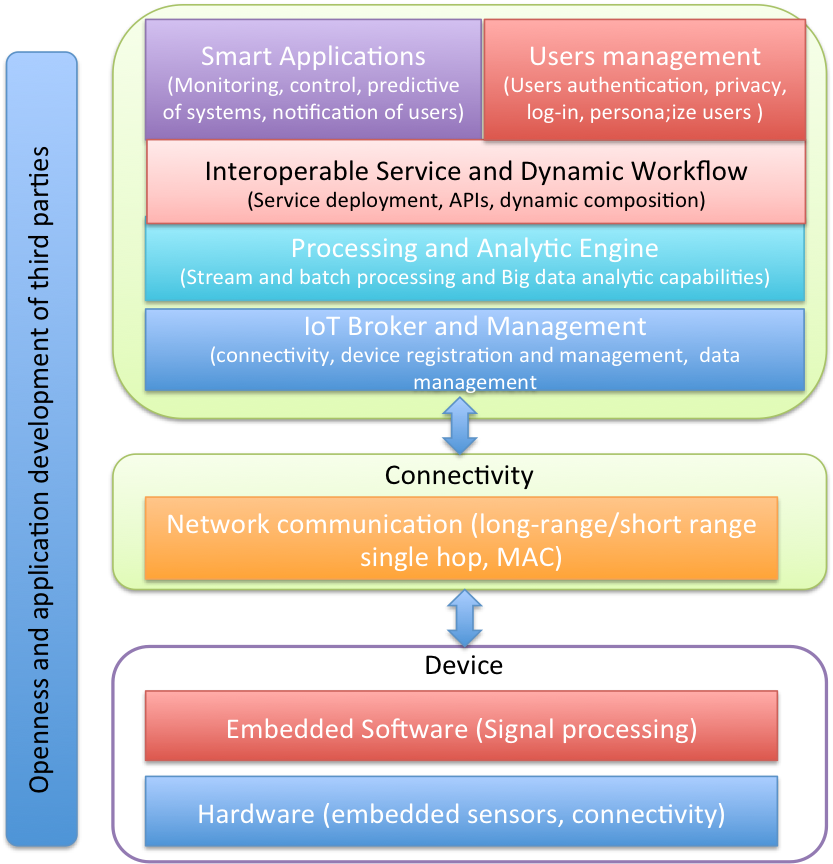
\includegraphics[width=0.7\textwidth]{figs/functional.png}
\caption{Functional overview of WAZIUP}
\label{fig:func}
\end{figure}

The Figure~\ref{fig:func} displays the functional overview of WAZIUP.
The topmost block represents the Cloud platform, the middle one is the network connectivity while the bottom one is the local deployment, including gateway and sensors.

\subsection{IoT platform}

\subsubsection{IoT architecture overview}

Our iot platform architecture is presented in Figure~\ref{fig:iotarchi}.
It has three main layers: device layer, gateway layer and the cloud layer.

\begin{figure}[h]
\centering
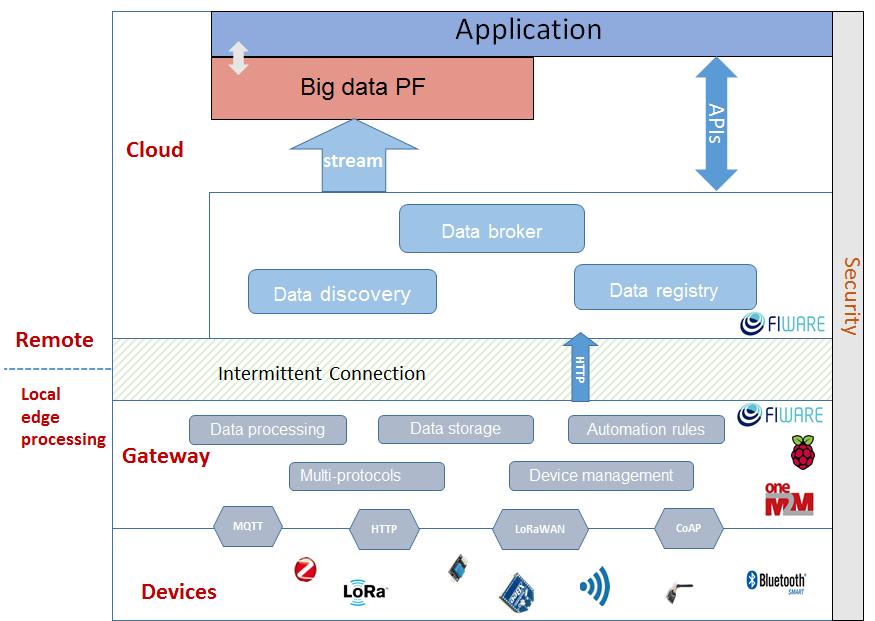
\includegraphics[width=\textwidth]{figs/iotarchi.png}
\caption{IoT platform architecture}
\label{fig:iotarchi}
\end{figure}



\begin{itemize}
  \item \emph{The device layer}
    It includes IoT sensors and actuator that are able to communicate each on its protocol (MQTT, CoAP, HTTP, LoRAWAN) with the gateway. 
It a constraint and autonomous device. 
Considering the project circumstances it has to be low cost and doesn’t consume much power.
  \item \emph{The gateway layer}
  The gateway is a key component in our architecture since it ensure a secure bidirectional communication between the Iot devices and the cloud services.
 It interfere with various kind of devices: getting the data from sensors and sending commands to actuators.
  It has to be multi-protocol in order to be able to support diverse devices and it need to have device management capabilities.
Since the connection is intermittent in our project, it is mandatory that the gateway is able to manage local rules (for example some event processing), to store data locally and to have low speed internet connectivity (2G: GPRS, EDGE).
  \item \emph{The cloud layer}
  Our cloud main component are: the Data broker, the data registry and the data discovery.
  \item \emph{Data broker:}
    it is the key component of the IoT cloud services, it is based on publish/ subscribe mechanism to ensure data transfer from different producers to their respected consumers.
  \item \emph{Data registry:}
    it contains the virtual representation of devices (the data and the meta-data)
  \item \emph{Data discovery:} 
    it is responsible on querying the data.
\end{itemize}


\subsubsection{Technology and tools}

In this section we will present the technology choices for each functional component stated above.
In the cloud level the functional component are the data broker, data registry and data discovery.
To cover these functionalities, The FIWARE generic enabler Orion context broker is the all-in-one solution.
It is based on the Next Generic Service Interfaces (NGSI) 9/10.
NGSI specification defines a data model and interfaces to manage the whole cycle of the virtual entities.  
We have also another candidate: the Nec IoT broker that cover the functionality of the data broker and that uses the ConfMan component for the data discovery and registry.
In the gateway level, we have these functionalities:

\begin{itemize}
    \item \emph{Multiprotocol}
The FIWARE IoT agent component: can be an option to ensure this characteristic. 
Each IoT agent can be responsible on the data transfer to and from the devices using the device specific protocol. 
    \item \emph{Device management}
We are considering the use of LwM2M device management protocol.
    \item \emph{Local rules}
FIWARE Cepheus enabler can be an option since it has a complex event processing engine. 
    \item \emph{Data processing}
this component will be developed depending on use cases requirements.
    \item \emph{Data storage}
Mongo DB can be an option, other light data bases can be also considered such as SQLiteDB.
\end{itemize}

In the devices and networking level, LoRa technology captured our attention. 
It specifies LoRaWAN for Low Power Wide Area Network (LPWAN), the kind of technology needed in our project context (rural environment). 
Using LoRaWAN we can reach above 20 km in Line-Of-Sight (LOS) condition between devices and the gateway. 


\subsection{Big Data Platform}

\todo{Charlotte}

\subsubsection{Big Data Platform overview}



